% XCircuit output "fly_simple.tex" for LaTeX input from fly_simple.eps
\def\putbox#1#2#3#4{\makebox[0in][l]{\makebox[#1][l]{}\raisebox{\baselineskip}[0in][0in]{\raisebox{#2}[0in][0in]{\scalebox{#3}{#4}}}}}
\def\rightbox#1{\makebox[0in][r]{#1}}
\def\centbox#1{\makebox[0in]{#1}}
\def\topbox#1{\raisebox{-0.60\baselineskip}[0in][0in]{#1}}
\def\midbox#1{\raisebox{-0.20\baselineskip}[0in][0in]{#1}}
   \scalebox{1}{
   \normalsize
   \parbox{5.36458in}{
   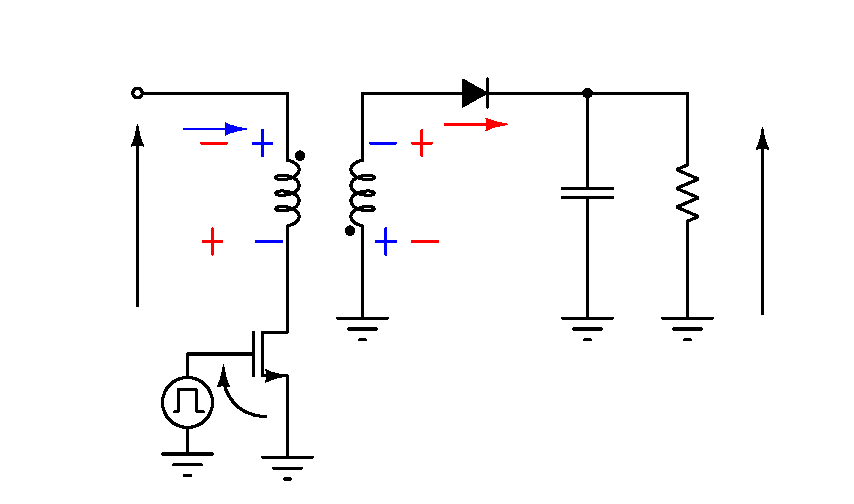
\includegraphics[scale=1]{fly_simple}\\
   % translate x=784 y=334 scale 0.38
   \putbox{4.09in}{1.91in}{1.20}{$R_S$}%
   \putbox{3.29in}{1.90in}{1.20}{$C_S$}%
   \putbox{2.97in}{2.88in}{1.20}{D}%
   \putbox{0.06in}{1.80in}{1.20}{$V_E$}%
   \putbox{1.47in}{1.96in}{1.20}{$L_1$}%
   \putbox{2.47in}{1.96in}{1.20}{$L_2$}%
   \putbox{1.35in}{0.30in}{1.20}{$V_{GS}$}%
   \putbox{3.20in}{2.70in}{1.20}{\textcolor{blue}{inversa}}%
   \putbox{3.18in}{2.94in}{1.20}{\textcolor{red}{directa}}%
   \putbox{1.97in}{0.82in}{1.20}{\textcolor{blue}{conduccion}}%
   \putbox{1.97in}{0.55in}{1.20}{\textcolor{red}{corte}}%
   \putbox{4.59in}{1.90in}{1.20}{$V_S$}%
   \putbox{2.87in}{2.21in}{1.20}{$I_D$}%
   \putbox{1.00in}{2.45in}{1.20}{$I_{L1}$}%
   } % close 'parbox'
   } % close 'scalebox'
   \vspace{-\baselineskip} % this is not necessary, but looks better
